\documentclass{article}
\usepackage[utf8]{inputenc}
\usepackage[polish]{babel}
\usepackage[T1]{fontenc}
\usepackage{graphicx}
\usepackage{float}
\usepackage[a4paper, left=3.7cm, right=3.7cm, top=3cm, bottom=2cm]{geometry}

\title{Projekt PAM - aplikacja służąca do rozwiązywania testów}
\author{Antoni Załupka}

\begin{document}
	\thispagestyle{empty}
	
	
	\vspace{4cm}
	
	\rule{\linewidth}{2mm} 
	
	\begin{center}
		\huge \textbf{Projektowanie Aplikacji Mobilnych} \\
		\huge {Aplikacja służąca do rozwiązywania quizów} \\
	\end{center}
	
	\rule{\linewidth}{0.5mm} 
	
	\vspace{2cm}
	
	\begin{center}
		\Large{Antoni Załupka} \\
		\Large{Numer indeksu: 351120} \\
		\Large{III rok, grupa PAW2} \\
		
	\end{center}
	
	
	\vspace{15cm}
	
	\begin{center}
		\Large{2025, Uniwersytet Śląski}
	\end{center}
	
	\newpage
	
	\tableofcontents
	
	\newpage
	
	\section{Wstęp}
	Celem niniejszego projektu było zaprojektowanie oraz zaimplementowanie mobilnej aplikacji edukacyjnej w formie quizów, przeznaczonej na urządzenia z systemem Android i stworzonej z wykorzystaniem technologii Flutter. Aplikacja wykorzystuje ten sam interfejs API co równolegle rozwijana wersja przeglądarkowa, zapewniając spójność działania i ułatwiając dalszy rozwój systemu.
	
	Quizy dostępne w aplikacji nie służą wyłącznie weryfikacji wiedzy użytkownika, lecz pełnią funkcję edukacyjną. Każde pytanie umożliwia niezwłoczne sprawdzenie poprawności odpowiedzi oraz jej modyfikację, co umożliwia naukę w oparciu o szybką informację zwrotną.
	
	W dalszej części sprawozdania będę używał nomenklatury stosowanej w oficjalnej dokumentacji Fluttera, gdzie znane z Androida \textit{aktywności} odpowiadają \textit{widżetom} oraz \textit{ekranom}.
	
	\subsection{Wymagania funkcjonalne}
	\begin{itemize}
		\item Możliwość logowania do aplikacji z wykorzystaniem danych uwierzytelniających oraz metod biometrycznych (odcisk palca);
		\item Pobieranie danych z API, w tym quizów oraz historii podejść użytkownika;
		\item Rozwiązywanie quizów i zapisywanie wyników;
		\item Przeglądanie historii podejść w dedykowanej zakładce;
		\item Możliwość wylogowania się z konta;
		\item Wsparcie dla języka polskiego oraz angielskiego.
	\end{itemize}
	
	\subsection{Wymagania niefunkcjonalne}
	\begin{itemize}
		\item Intuicyjny i przejrzysty interfejs użytkownika;
		\item Wysoka responsywność aplikacji na różnych urządzeniach z systemem Android;
		\item Bezpieczna obsługa danych użytkownika (uwierzytelnianie biometryczne, bezpieczne przechowywanie tokenów dostępowych JWT);
		\item Wydajna komunikacja z API (minimalizacja liczby zapytań);
		\item Utrzymanie spójności z wersją webową.
	\end{itemize}

\section{Specyfikacja zewnętrzna}
Aplikacja charakteryzuje się przejrzystością oraz prostotą obsługi. W tej sekcji postaram się zobrazować najważniejsze elementy interfejsu użytkownika w punktach. Obok każdego punktu (z wyłączeniem punktu 1.) znajduje się rysunek poglądowy.
\begin{enumerate}
\item \textbf{Instalacja aplikacji:} \\
\begin{itemize}
	\item Aplikację (na chwilę prezentacji) można pobrać ze strony \\ \texttt{https://quiz.azalupka.cc/mobile}. \\ Możliwe jest również samodzielne zbudowanie pliku instalacyjnego (\texttt{.apk}).
\end{itemize}
\item \textbf{Ekran powitalny:} \\
	\begin{minipage}{0.5\textwidth}
		\begin{itemize}
			\item Po uruchomieniu aplikacji wyświetlane jest logo oraz przycisk logowania.
			\item Przycisk logowania umożliwia przejście do dalszych funkcji aplikacji.
		\end{itemize}
	\end{minipage}
	\begin{minipage}{0.5\textwidth}
		\begin{figure}[H]
			\centering
			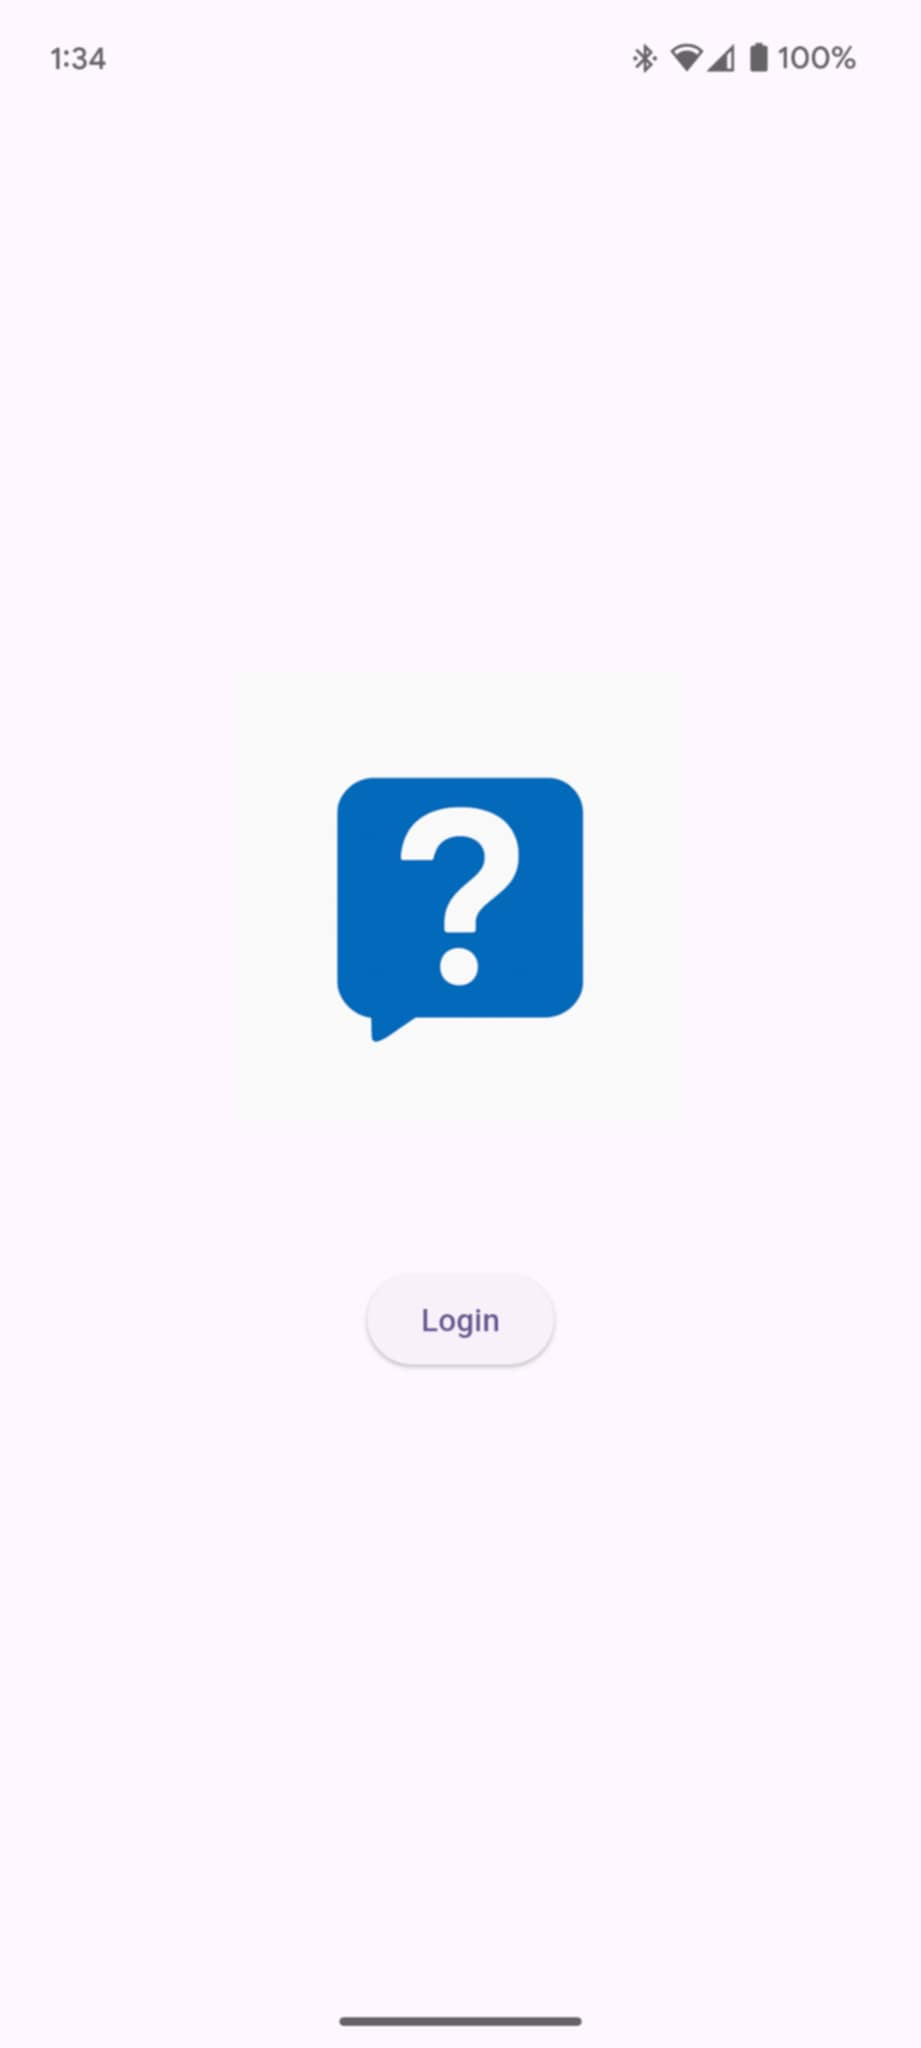
\includegraphics[width=0.5\textwidth]{../_assets/mobile/welcome.jpeg}
			\caption{Ekran powitalny aplikacji}
			\label{fig:welcome}
		\end{figure}
	\end{minipage}
\item \textbf{Logowanie:} \\
	\begin{minipage}{0.5\textwidth}
		\begin{itemize}
			\item Proces logowania polega na podaniu adresu e-mail oraz hasła, a następnie zatwierdzeniu danych.
			\item W przypadku urządzeń obsługujących biometrię oraz wcześniejszego logowania, dostępna jest opcja logowania odciskiem palca.
		\end{itemize}
	\end{minipage}
	\begin{minipage}{0.5\textwidth}
		\begin{figure}[H]
			\centering
			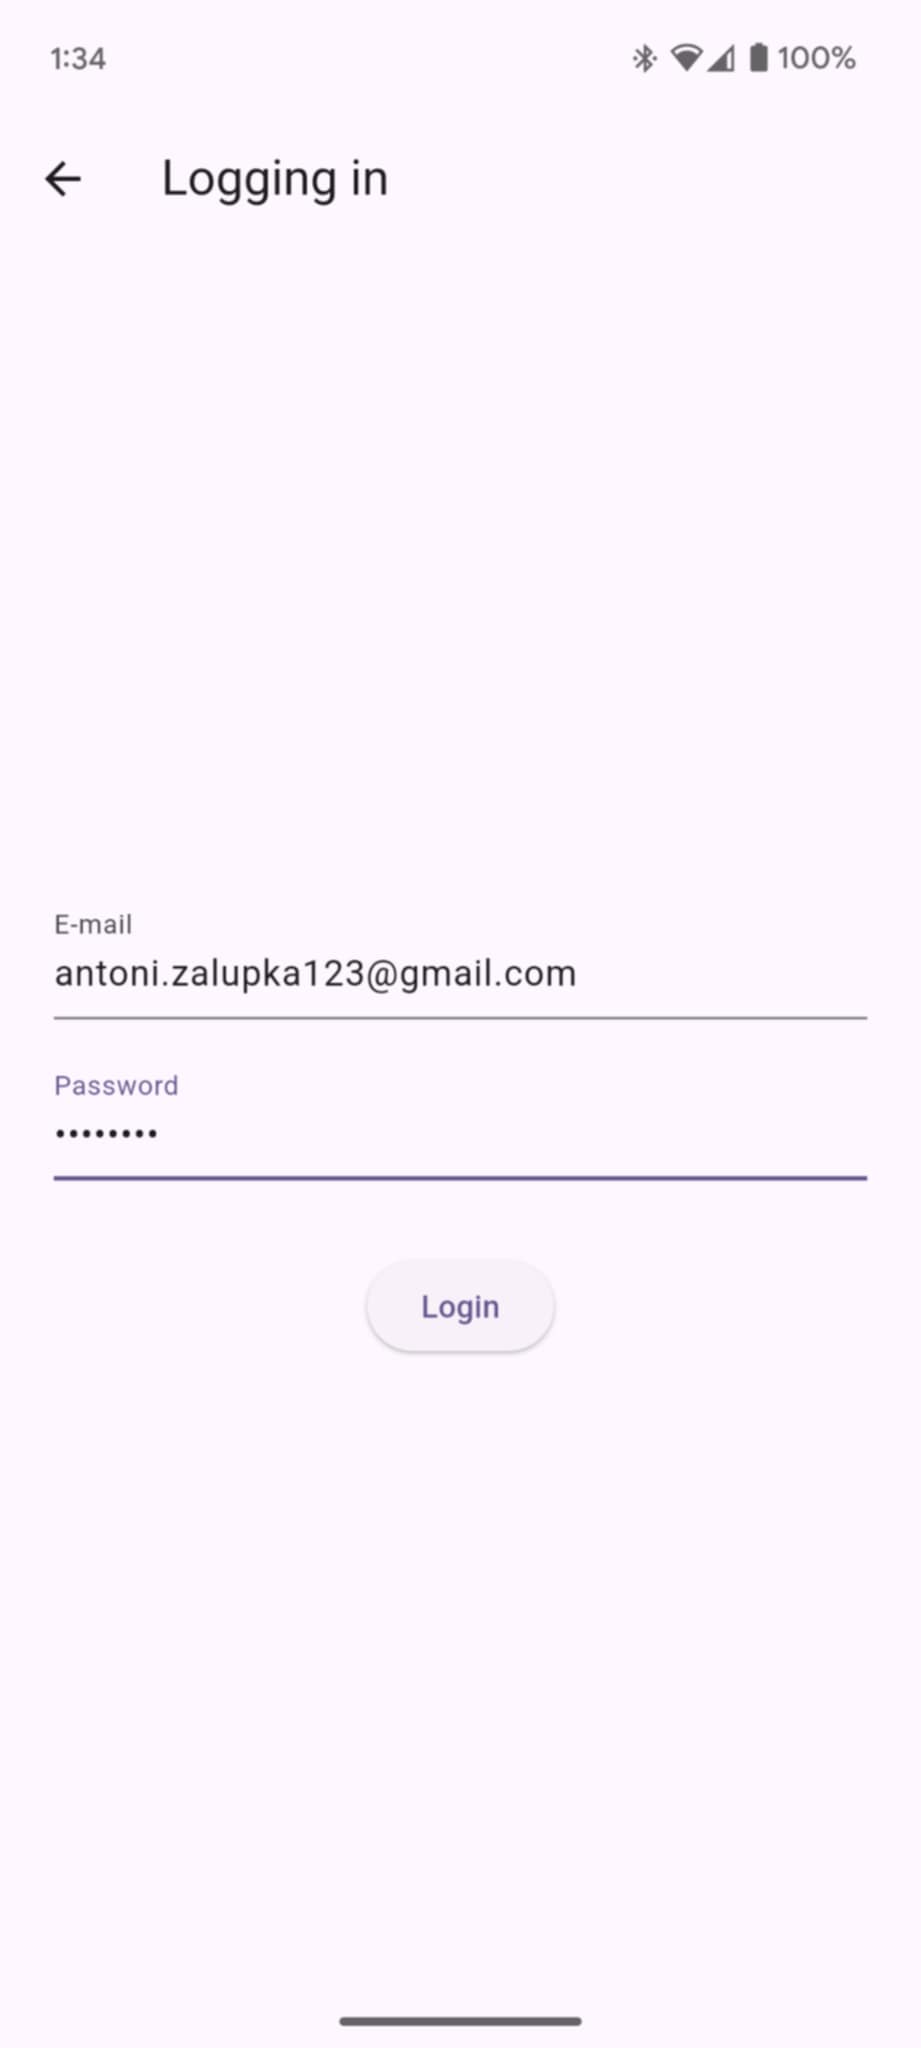
\includegraphics[width=0.5\textwidth]{../_assets/mobile/login_filled.jpeg}
			\caption{Ekran logowania (pierwsze logowanie)}
			\label{fig:login_filled}
		\end{figure}
	\end{minipage}
\item \textbf{Przeglądanie quizów:} \\
	\begin{minipage}{0.5\textwidth}
		\begin{itemize}
			\item Po zalogowaniu prezentowana jest lista dostępnych quizów.
			\item Rozpoczęcie podejścia do wybranego quizu następuje po wybraniu przycisku „Start” na odpowiedniej karcie.
		\end{itemize}
	\end{minipage}
	\begin{minipage}{0.5\textwidth}
		\begin{figure}[H]
			\centering
			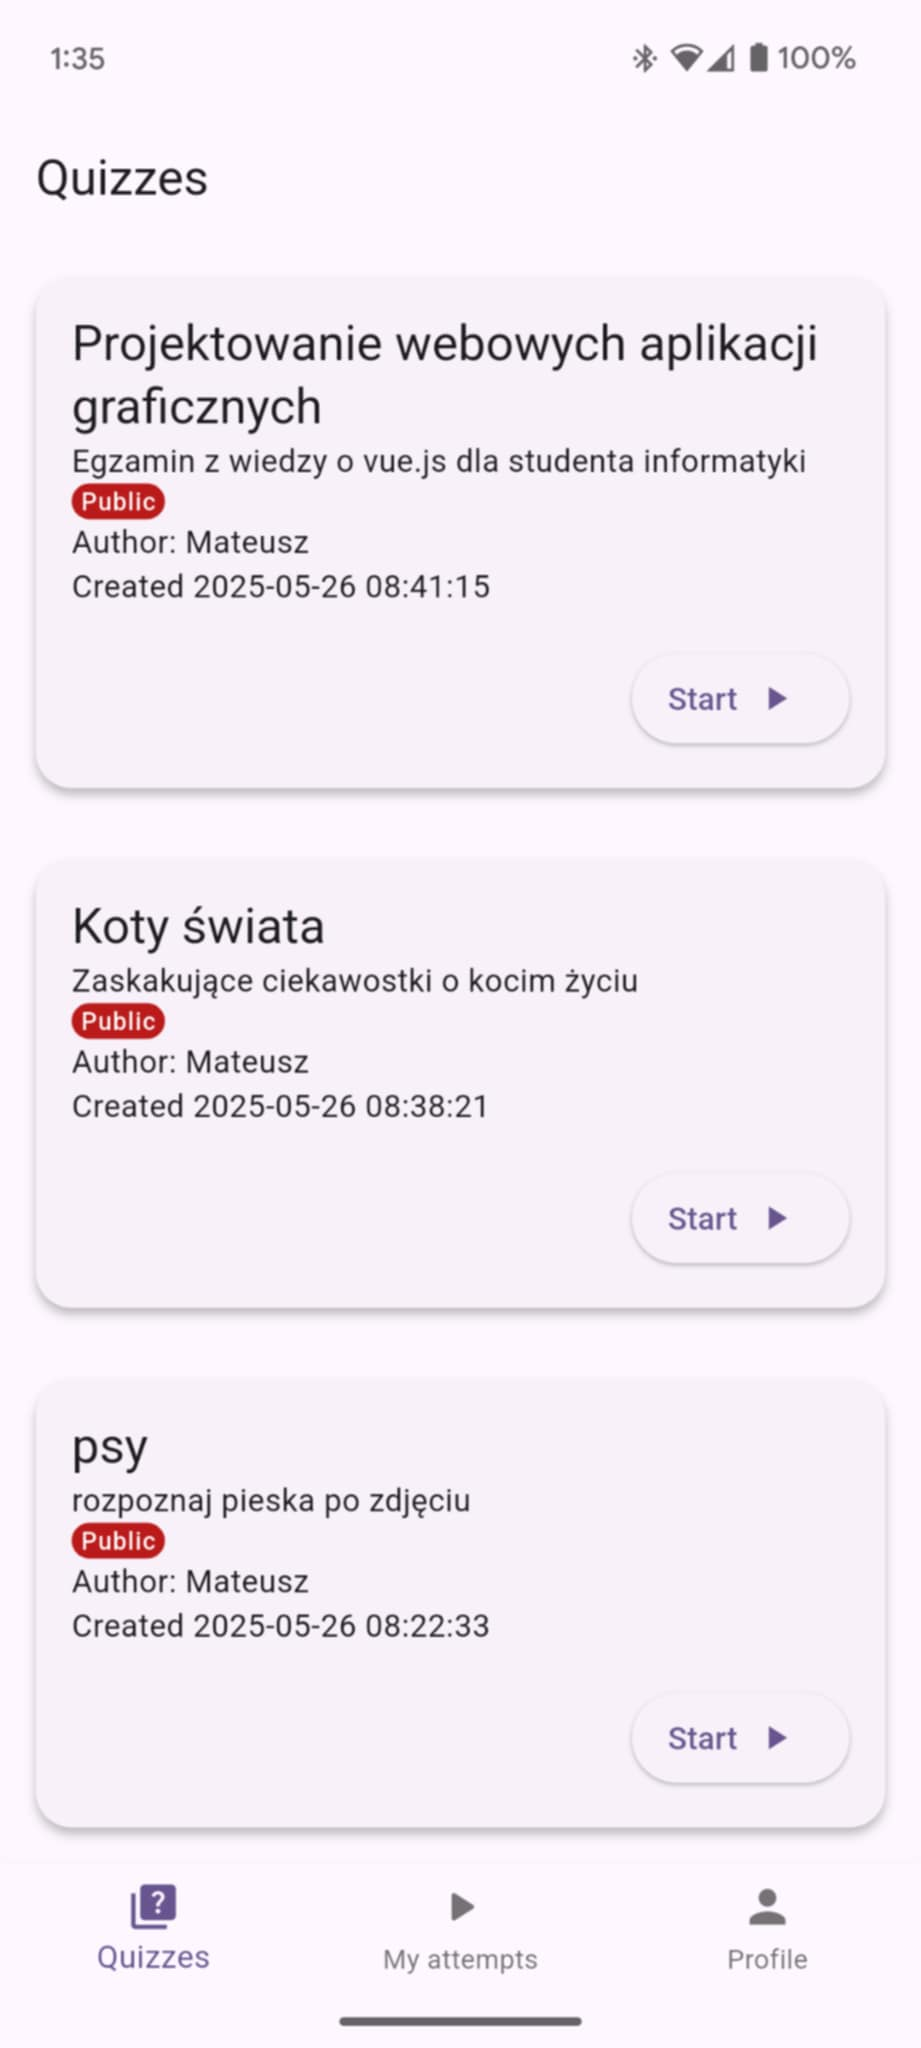
\includegraphics[width=0.5\textwidth]{../_assets/mobile/quizzes.jpeg}
			\caption{Ekran listy dostępnych quizów}
			\label{fig:quizzes}
		\end{figure}
	\end{minipage}
\item \textbf{Rozwiązywanie quizu:} \\
	\begin{minipage}{0.5\textwidth}
		\begin{itemize}
			\item Każde pytanie prezentowane jest osobno.
			\item Odpowiedzi zaznaczane są poprzez wybór odpowiedniego pola wyboru.
			\item Podgląd prawidłowych odpowiedzi dostępny jest po wybraniu ikony oka w prawym górnym rogu pytania.
			\item Wynik aktualizowany jest na bieżąco na dole ekranu, a pasek procentowy prezentuje odsetek poprawnych odpowiedzi.
		\end{itemize}
	\end{minipage}
	\begin{minipage}{0.5\textwidth}
		\begin{figure}[H]
			\centering
			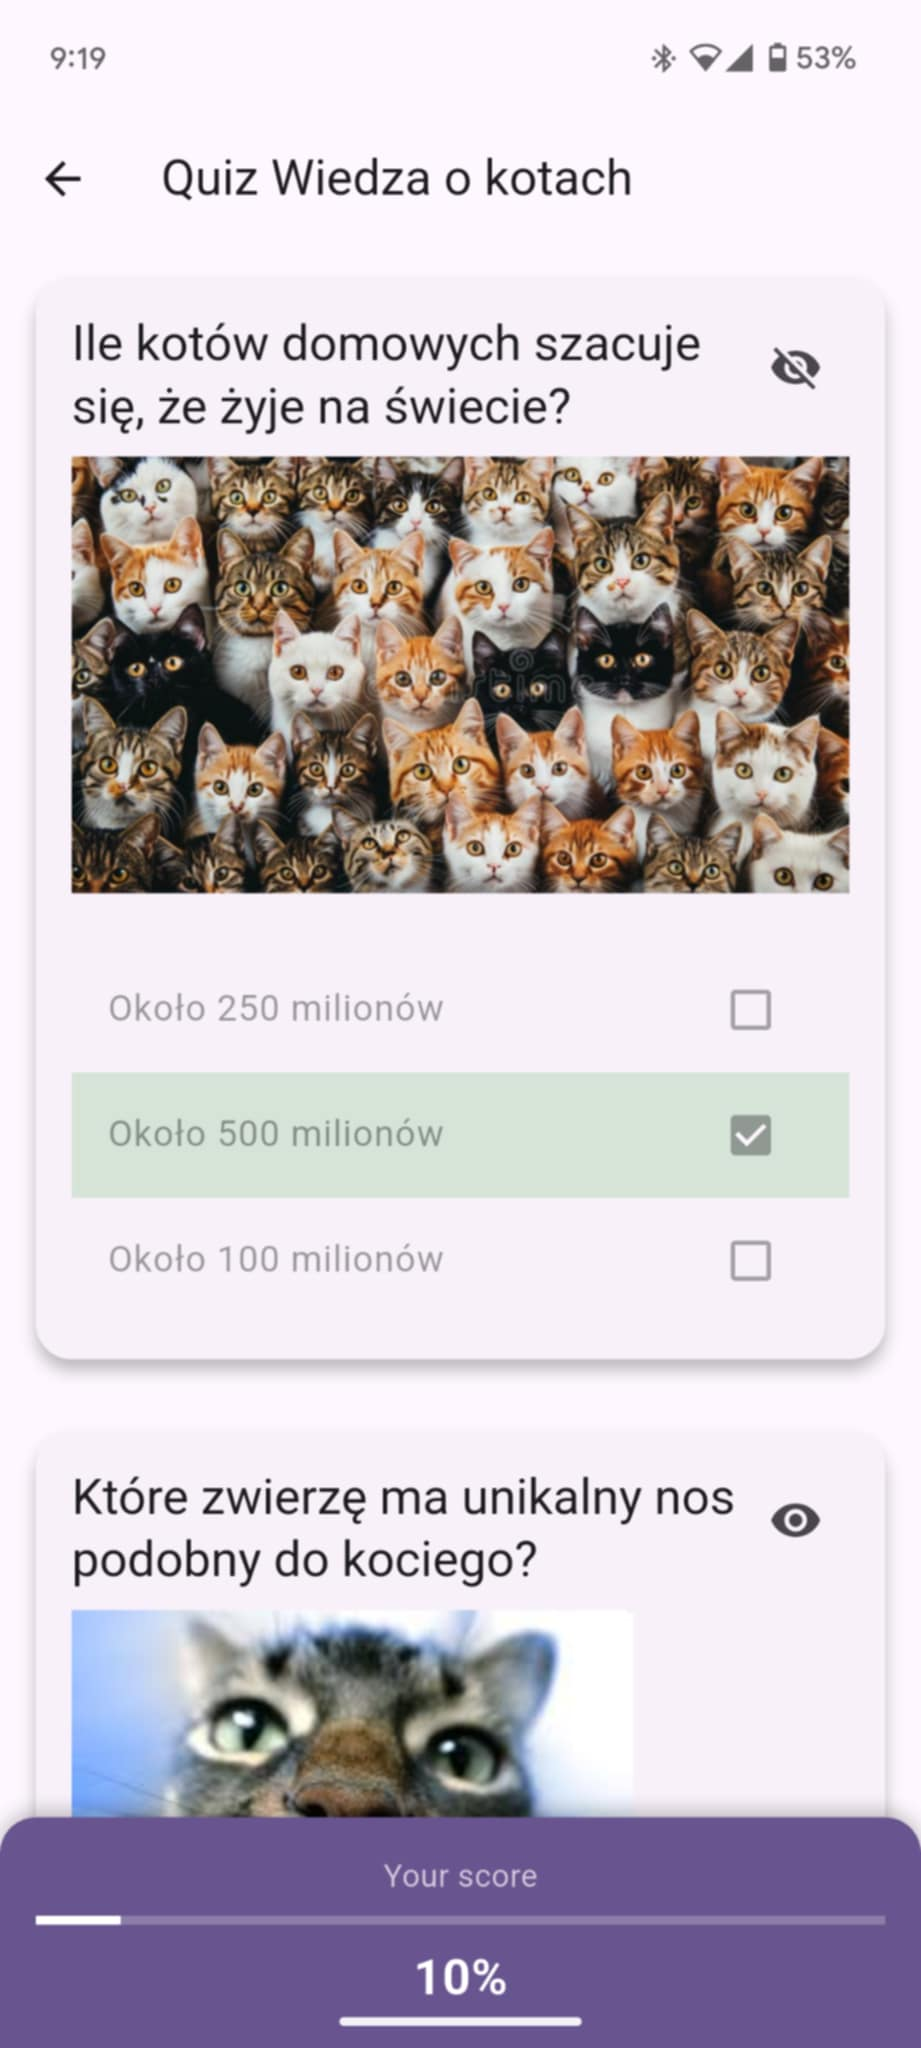
\includegraphics[width=0.5\textwidth]{../_assets/mobile/attempt.jpeg}
			\caption{Ekran podejścia do quizu}
			\label{fig:attempt}
		\end{figure}
	\end{minipage}
\item \textbf{Historia podejść:} \\
	\begin{minipage}{0.5\textwidth}
		\begin{itemize}
			\item Zakładka „Moje podejścia” na dolnym pasku nawigacji umożliwia przeglądanie historii quizów wraz z wynikami.
			\item Dostępne są opcje rozpoczęcia nowego podejścia lub kontynuacji poprzedniego.
		\end{itemize}
	\end{minipage}
	\begin{minipage}{0.5\textwidth}
		\begin{figure}[H]
			\centering
			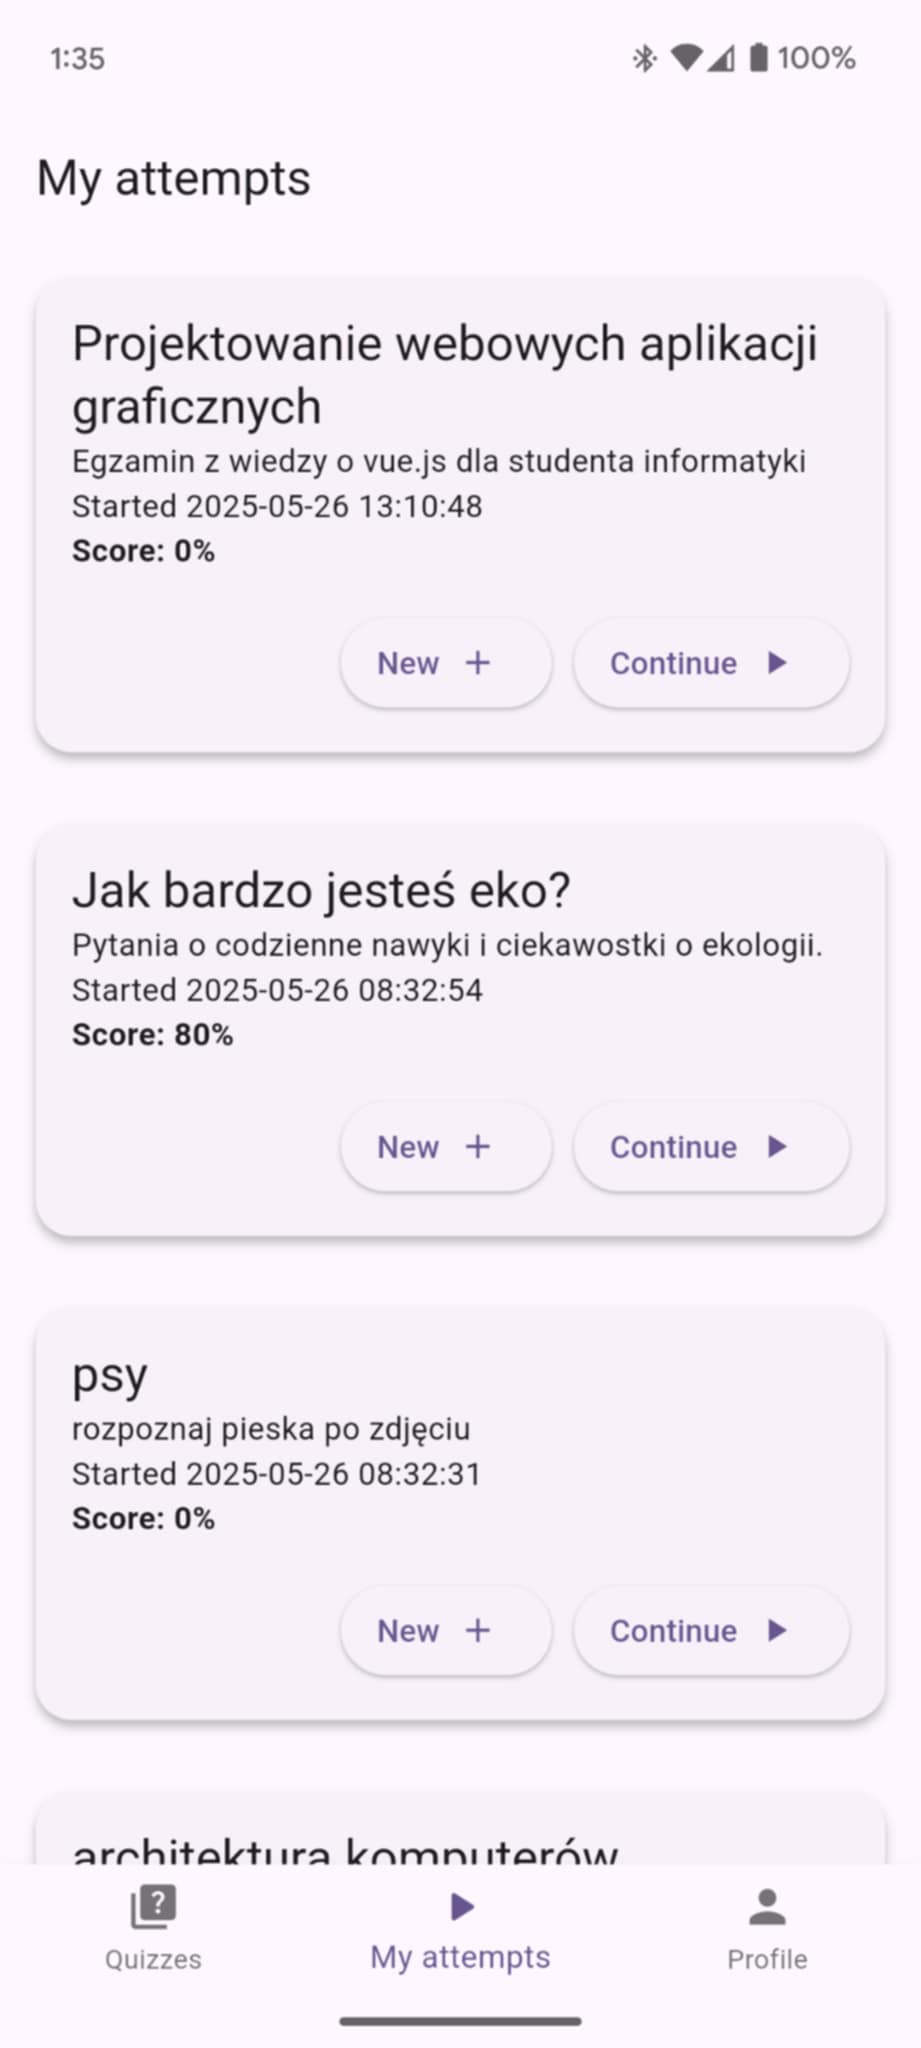
\includegraphics[width=0.5\textwidth]{../_assets/mobile/attempts.jpeg}
			\caption{Ekran historii podejść}
			\label{fig:attempts}
		\end{figure}
	\end{minipage}
\item \textbf{Profil i wylogowanie:} \\
	\begin{minipage}{0.5\textwidth}
		\begin{itemize}
			\item W zakładce „Profil” prezentowane są podstawowe informacje o użytkowniku oraz dostępny jest przycisk wylogowania.
			\item Wylogowanie powoduje zakończenie bieżącej sesji.
		\end{itemize}
	\end{minipage}
	\begin{minipage}{0.5\textwidth}
		\begin{figure}[H]
			\centering
			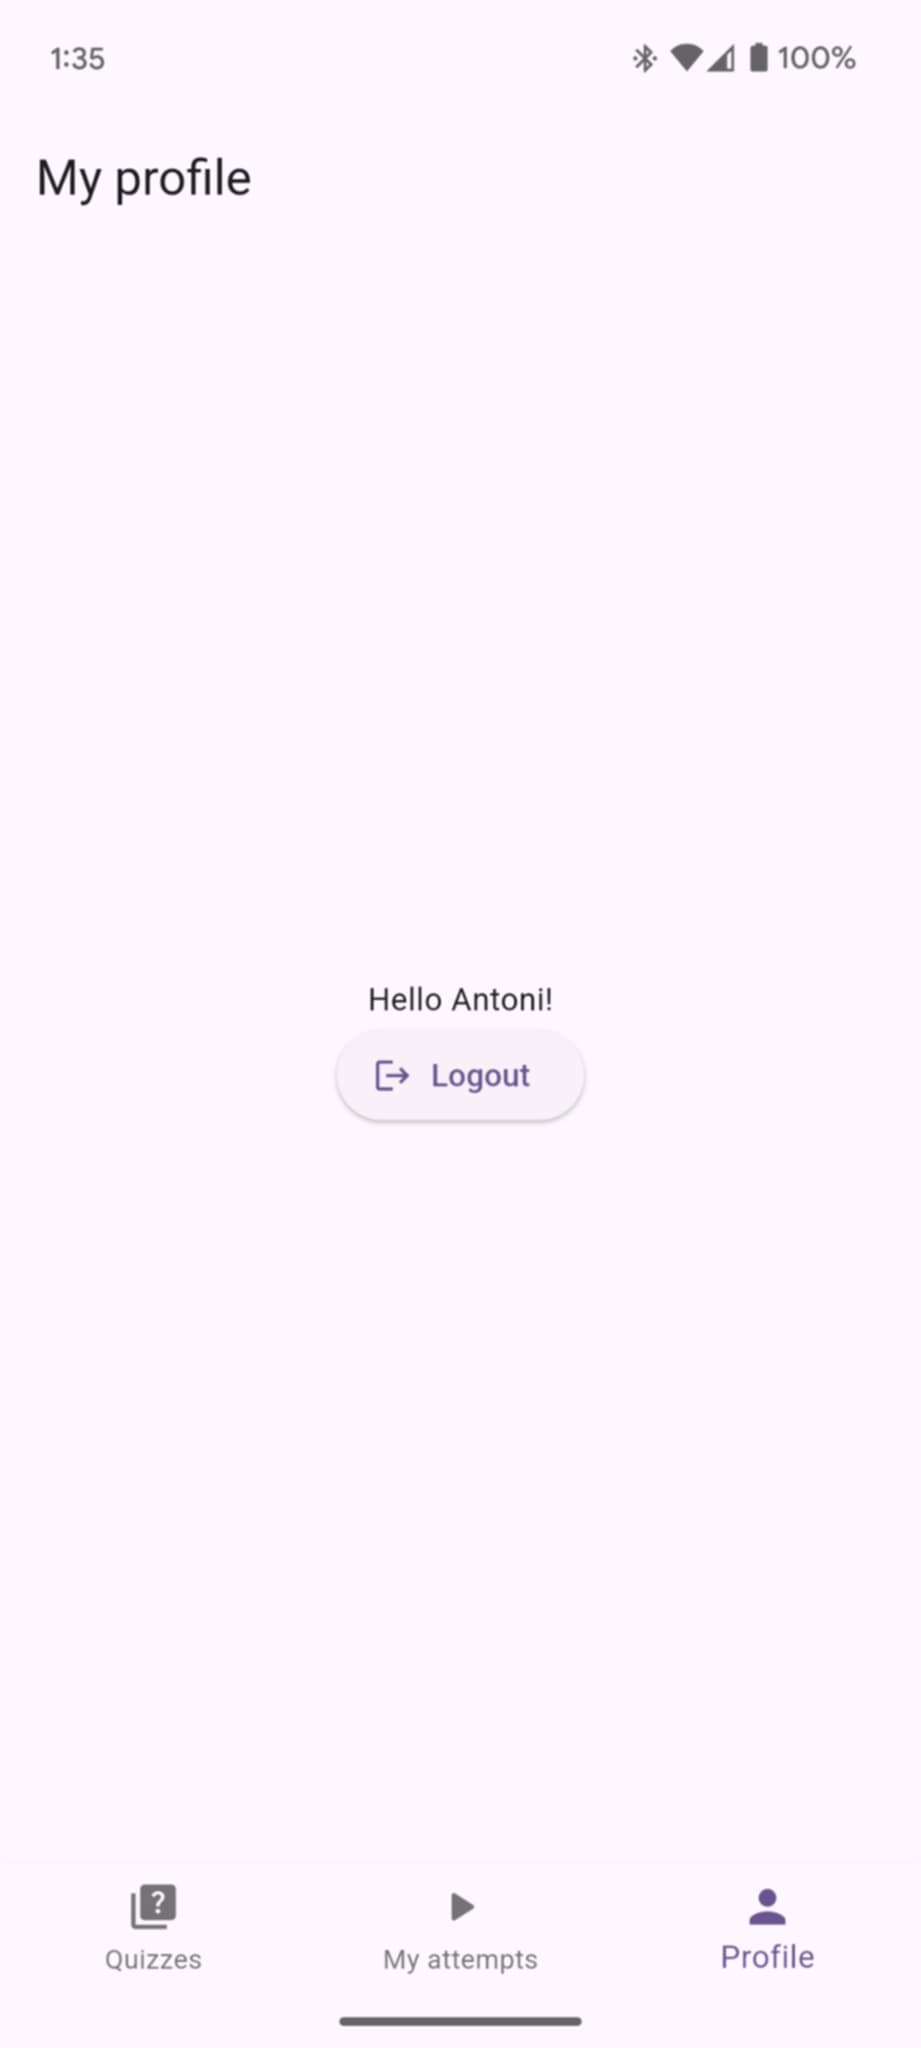
\includegraphics[width=0.5\textwidth]{../_assets/mobile/profile.jpeg}
			\caption{Ekran profilu}
			\label{fig:profile}
		\end{figure}
	\end{minipage}
\end{enumerate}

\section{Specyfikacja wewnętrzna}
	Aplikacja mobilna została zrealizowana w technologii Flutter, z wykorzystaniem architektury opartej na podziale na warstwy prezentacji, logiki biznesowej oraz dostępu do danych. Struktura projektu umożliwia łatwą rozbudowę oraz modyfikację przez innych programistów.

	\subsection{Struktura aplikacji}
		Kod źródłowy podzielony jest na warstwy, którym odpowiadają katalogi na dysku:
		\begin{itemize}
			\item \textbf{Warstwa prezentacji} – komponenty interfejsu użytkownika (ekrany – widżety, m.in.: ekrany logowania, quizów, profilu, historii podejść);
			\item \textbf{Warstwa komunikacji} – serwisy komunikujące się z API GraphQL (m.in.: \texttt{AuthService}, \texttt{QuizService}, \texttt{QuestionService});
			\item \textbf{Modele danych} – na ich podstawie serwisy tworzą obiekty z pozyskanych z backendu danych (\texttt{UserModel}, \texttt{Quiz}, \texttt{QuizAttempt}, \texttt{Question}, \texttt{Answer});
			\item \textbf{Stan aplikacji} – większość widżetów posiada własny stan, aplikacja zawiera jeden provider służący do przechowywania danych obecnie zalogowanego użytkownika (\texttt{UserProvider});
			\item \textbf{l10n} – paczki językowe (języki: polski i angielski).
		\end{itemize}

	\subsection{Główne elementy aplikacji}
		\begin{itemize}
			\item \textbf{Ekrany (Screens):} Grupują widżety, aby zapewnić użytkownikowi praktyczny interfejs. Przykładowe ekrany: \texttt{LoginScreen}, \texttt{QuizzesScreen}, \texttt{AttemptsScreen}, \texttt{ProfileScreen}, \texttt{AttemptScreen}. Nawigacja odbywa się za pomocą \texttt{BottomNavigationBar} oraz \texttt{Navigator}.
			\item \textbf{Widżety (Widgets):} Komponenty takie jak \texttt{QuizCard}, \texttt{QuizAttemptCard}, \texttt{QuestionCard} odpowiadają za prezentację pojedynczych quizów, podejść oraz pytań.
			\item \textbf{Provider:} Do zarządzania stanem zalogowanego użytkownika wykorzystano wzorzec Provider (\texttt{UserProvider}), co umożliwia łatwy dostęp do danych użytkownika w całej aplikacji.
			\item \textbf{Serwisy:} Warstwa serwisów odpowiada za komunikację z backendem poprzez GraphQL. Każdy serwis (np. \texttt{QuizService}, \texttt{QuizAttemptService}, \texttt{QuestionService}) posiada metody do pobierania i zapisywania danych. W GraphQL są to odpowiednio \textbf{queries} oraz \textbf{mutations}.
			\item \textbf{Modele danych:} Każdy typ danych pobierany z API posiada swój model z metodami serializacji i deserializacji.
		\end{itemize}

	\subsection{Wykorzystane API i biblioteki}
		\begin{itemize}
			\item \textbf{Flutter} – framework do budowy aplikacji mobilnych;
			\item \textbf{graphql\_flutter} – obsługa zapytań i mutacji GraphQL do backendu;
			\item \textbf{provider} – przechowywanie stanu z danymi zalogowanego użytkownika w całej aplikacji;
			\item \textbf{local\_auth} – obsługa biometrii (odcisk palca);
			\item \textbf{flutter\_secure\_storage} – bezpieczne przechowywanie tokenu JWT i danych użytkownika;
			\item \textbf{intl, flutter\_localizations} – obsługa wielu języków.
		\end{itemize}

	\subsection{Informacje dotyczące kodu i uruchamiania}
		\begin{itemize}
			\item Przed uruchomieniem należy skonfigurować w pliku \texttt{lib/main.dart} poprawny adres backendu poprzez edycję następującej linijki: \\
			\texttt{AuthService().initClient("https://apiquiz.azalupka.cc");}
			\item Do uruchomienia aplikacji wymagane jest środowisko Flutter (zalecana wersja SDK zgodna z \texttt{pubspec.yaml}).
			\item Aby uruchomić aplikację na emulatorze lub urządzeniu fizycznym, należy wykonać polecenie \texttt{flutter run} w katalogu projektu.
			\item Do budowy pliku APK służy polecenie \texttt{flutter build apk}.
		\end{itemize}

	Aplikacja została zaprojektowana w sposób umożliwiający łatwe dodawanie nowych funkcji, ekranów oraz integrację z innymi usługami backendowymi.

\section{Wnioski}
\subsection{Obsługa biometrii}
	Pierwszym wyzwaniem podczas realizacji projektu było poprawne wykrywanie, czy urządzenie wspiera logowanie biometryczne (np. odcisk palca). Wymagało to zapoznania się z biblioteką \texttt{local\_auth} oraz obsługą różnych przypadków, gdy urządzenie nie posiada odpowiedniego sprzętu lub użytkownik nie skonfigurował biometrii.
	
	\subsection{Integracja z API GraphQL}
	Drugim istotnym problemem była integracja z API GraphQL, szczególnie że wcześniej nie miałem doświadczenia z językiem Dart w praktyce. Początkowo pojawiały się trudności z autoryzacją oraz poprawnym zapisem i odczytem tokena JWT we \texttt{flutter\_secure\_storage}. Problemy te zostały rozwiązane przez ujednolicenie kontekstu zapytań GraphQL (z użyciem \texttt{Context.fromList}) oraz weryfikację nagłówków zwracanych w odpowiedzi. Ponadto w funkcjach pobierających dane dodałem sprawdzenie \texttt{context.mounted} przed dokonaniem nawigacji lub aktualizacją stanu, co wyeliminowało wyjątki związane z odmontowaniem widżetu.
	
	\subsection{Projektowanie interfejsu w Flutterze}
	Dodatkowym wyzwaniem okazało się projektowanie interfejsu użytkownika we Flutterze, który znacząco różni się od podejścia znanego mi z HTML i CSS. Tworzenie widżetów oraz układów wymagało przestawienia się na deklaratywny sposób budowania interfejsu oraz zrozumienia hierarchii widgetów, co początkowo było nieintuicyjne w porównaniu do stylowania stron internetowych.
	
	\subsection{Obsługa wielu języków}
	Na końcowym etapie projektu zdecydowałem się dodać obsługę wielu języków. W tym celu wykorzystałem mechanizm lokalizacji Fluttera oraz pliki \texttt{.arb} z tłumaczeniami (angielski i polski). W kodzie aplikacji pojawiły się wywołania takie jak \\
	\texttt{AppLocalizations.of(context)!.login}, \\
	które dynamicznie pobierają odpowiednie tłumaczenie w zależności od ustawień systemowych użytkownika. Dzięki temu aplikacja automatycznie dostosowuje się do języka urządzenia, a dodanie kolejnych tłumaczeń sprowadza się do edycji plików w katalogu \texttt{lib/l10n}.

	\vspace{0.3cm}

W perspektywie dalszego rozwoju możliwe byłoby:
\begin{itemize}
  \item Wprowadzenie trybu offline z lokalnym cache’em quizów i wyników,
  \item Rozszerzenie typów pytań,
  \item Integracja powiadomień push do przypominania o nowych quizach,
  \item Panel administracyjny do zarządzania treścią quizów i kontami użytkowników bezpośrednio w aplikacji,
  \item Wprowadzenie obsługi motywów graficznych.
\end{itemize}

Implementacja tego projektu dostarczyła cennych doświadczeń w zakresie architektury aplikacji Flutter, pracy z GraphQL oraz zarządzania stanem użytkownika.

\end{document}